\documentclass{jsarticle}
\usepackage{amsmath, smssymb, amsfonts}
\usepackage{newtxtext, newtxmath}
\usepackage{latexsym}
\usepackage{mathrsfs}
\usepackage{mathtools}
\usepackage{textcomp}
\usepackage{mathcomp}
\usepackage[dvipdfmx]{graphicx, xcolor}
\usepackage{float}
\usepackage{wrapfig}	% must be after float package.
\usepackage{subcaption}
\usepackage{booktabs}
\usepackage{url}
\usepackage{listings, jvlisting, color}

\definecolor{OliveGreen}{rgb}{0.0,0.6,0.0}
\definecolor{Orenge}{rgb}{0.89,0.55,0}
\definecolor{SkyBlue}{rgb}{0.28, 0.28, 0.95}
\lstset{
  language={C++}, % 言語の指定
  basicstyle={\ttfamily},
  identifierstyle={\small},
  commentstyle={\smallitshape},
  keywordstyle={\small\bfseries},
  ndkeywordstyle={\small},
  stringstyle={\small\ttfamily},
  frame={tb},
  breaklines=true,
  columns=[l]{fullflexible},
  numbers=left,
  xrightmargin=0zw,
  xleftmargin=3zw,
  numberstyle={\scriptsize},
  stepnumber=1,
  numbersep=1zw,
  lineskip=-0.5ex,
  keywordstyle={\color{SkyBlue}},     %キーワード(int, ifなど)の書体指定
  commentstyle={\color{OliveGreen}},  %注釈の書体
  stringstyle=\color{Orenge}          %文字列
}


\begin{document}

\title{ゼミ レポート}
\author{山田朔也}
\maketitle

\section{本レポートについて}
本レポートは6月7日に行われたゼミにて出題された課題に対するレポートなっている。
課題の内容は、Permalloy膜のような強磁性体薄膜において、
膜厚が有限の場合における1次元磁壁の磁化構造を求めるプログラムを作成することとなる。

\section{原理}
\subsection{膜厚有限の場合の1次元磁壁の磁化構造計算の特徴}
膜厚有限の場合は、無限の場合と異なり、静磁界の計算を解析的に行うことができない。
そのため、静磁界の計算は数値計算で行うことが必要となる。

\subsection{Permalloy膜の特徴}
Permalloy膜のような面内異方性が非常に弱く強磁性膜はある特徴を持つ。

原子磁気モーメントが膜厚方向に構造を持たず、磁化容易軸をy方向とする。
そのとき磁壁の構造は以下の図\ref{fig01},\ref{fig02}のいずれかのような構造となる。
\begin{figure}[H]
	\centering
	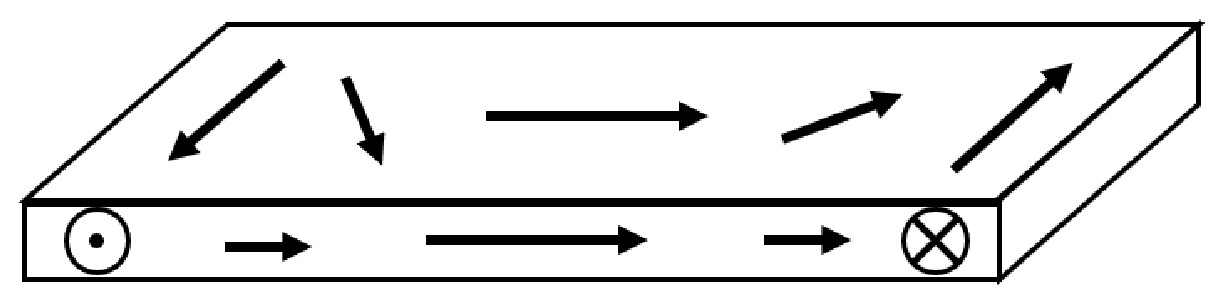
\includegraphics[width=14cm]{pic01.eps}
	\caption{1次元$\mathrm{N\Acute{e}el}$磁壁}
	\label{fig01}
\end{figure}
\begin{figure}[H]
	\centering
	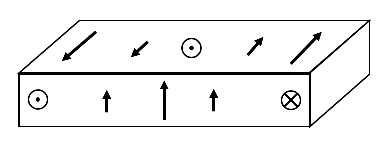
\includegraphics[width=14cm]{pic02.eps}
	\caption{1次元Bloch磁壁}
	\label{fig02}
\end{figure}

ただし現実の薄膜では、膜の厚さ方向にも原子磁気モーメントを持つ構造が現れる。
しかし、計算の単純化のため、今回は上図の1次元磁壁から計算を始めることとする。

\subsubsection{Bloch磁壁}
この磁壁では、磁壁の中心部で原子磁気モーメントが膜の厚さ方向を向くため、
磁壁中心部の膜の上下面に磁極が現れる。
これによって磁壁中心部に原子磁気モーメントの向きと反対方向の静磁界が現れる。
膜厚が薄いとき、磁極が近づくため静磁界が大きくなり、静磁エネルギーが増加する。
このエネルギーを小さくするため、磁壁幅は狭くなる。
また、異方性エネルギーも同様に磁壁幅が狭いほうがエネルギーは減少する。
しかし、磁壁幅が狭くなると交換エネルギーは増加する。
Bloch磁壁の磁壁幅はこれらのエネルギーの釣り合いによって決定づけられる。

\subsubsection{$\mathrm{N\Acute{e}el}$磁壁}
$\mathrm{N\Acute{e}el}$磁壁は、膜厚が非常に薄くなった時に現れる。
つまり、膜厚が一定以上薄くなった時に、Bloch磁壁の構造を維持できなくなることにより発生する。
この磁壁では、磁極は膜の内部で原子磁気モーメントの向きが変わるところに現れる。
局所的に大きな磁極が現れると静磁エネルギーは増大するため、
これを減少させるため磁壁幅は広くなる。
また、それによって交換エネルギーは減少する。
磁壁の幅を薄くする方向に働くのはこれら以外の効果である異方性エネルギーだけとなる。
しかし、今回考えるPermalloy膜の異方性エネルギーは非常に小さいため、$\mathrm{N\Acute{e}el}$
磁壁の幅は、Bloch磁壁に比べ非常に大きくなる。

\subsection{静磁界計算}
対象とする計算領域は、同じ大きさの長方形セルで離散化し、
磁気モーメントは各セルの中心にあるとする。
ここで、一つの長方形領域内での原子磁気モーメントの向きは、
その領域の中心点での原子磁気モーメントと同じ方向と仮定する。
この仮定により、計算領域内での磁荷は前述の長方形の辺にのみ現れることになる。
次に、長方形の各辺に現れる磁極が作り出す静磁界を求める方法を見ていく。

計算領域内の一つの長方形の辺と磁界観測点との関係は、図\ref{fig03}のようになる。
\begin{figure}[H]
	\centering
	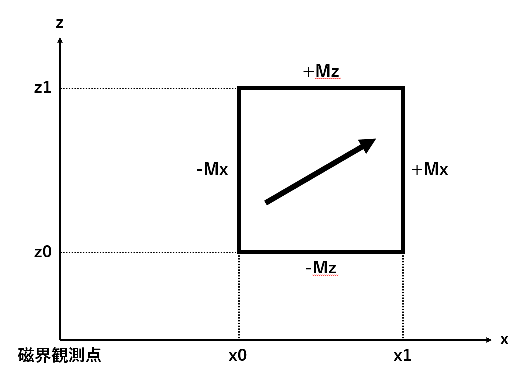
\includegraphics[width=14cm]{pic03.eps}
	\caption{静磁界の計算}
	\label{fig03}
\end{figure}
長方形の各辺は、それぞれ面密度$\pm Mx$および$\pm Mz$で磁極が分布している。
これらの辺に現れる磁極が観測点に作る静磁界を求める。

まずz軸に平行な右側の辺について考える。
対象とする構造はy方向に無限に同じ構造が続いている2次元構造であるため、直線状に一様に磁極が分布したモデルが適用できる。
よって、観測点から$(x1,z)$離れた対象返上の微小領域が作る磁界は
\begin{align}
	&\Delta Hx = -\frac{2}{\sqrt{x1^2 + z^2}} \frac{x1}{\sqrt{x1^2 + z^2}}Mx\Delta z	\label{01}	\\
	&\Delta Hz = -\frac{2}{\sqrt{x1^2 + z^2}}\frac{z}{\sqrt{x1^2 + z^2}}Mx\Delta z	\label{02}	
\end{align}
となる。

対象辺の磁極が観測点に作り出す磁界は、これらの式を辺に沿って積分することにより求められる。
\begin{align}
	Hx = &-2\int_{z0}^{z1}\frac{x1}{x1^2+z^2}Mx\,dz = -2Mx\left(\tan^{-1}\frac{z1}{x1} - \tan^{-1}\frac{z0}{x1}\right),	\label{03} \\
		  &\left(-\frac{\pi}{2} \leq \frac{z1}{x1} \leq \frac{\pi}{2} , -\frac{\pi}{2} \leq \frac{z0}{x1} \leq \frac{\pi}{2} \right) \notag	\\
	Hz = &-2\int_{z0}^{z1}\frac{z}{x1^2+z^2}Mx\,dz = -Mx\left[\log\left(x1^2+z1^2\right) - \log\left(x1^2+z0^2\right)\right]	\label{04}
\end{align}
z軸に平行なもう一方の辺の磁極が作る磁界も、同様にして求めることができる。
これら2つの辺が観測点に作る磁界は
\begin{align}
	Hx = &-2Mx\left(\tan^{-1}\frac{z1}{x1} - \tan^{-1}\frac{z1}{x0} - \tan^{-1}\frac{z0}{x1} + \tan^{-1}\frac{z0}{x0}\right) = qxx\cdot mx	\label{05} \\
		 &\left(\text{但し}\frac{z1}{x1},\frac{z1}{x0},\frac{z0}{x1},\frac{z0}{x0} \text{は} -\frac{2}{\pi} \text{から} \frac{2}{\pi} \text{の値} \right) \notag \\
	Hz = &-Mx\left[\log\left(x1^2+z1^2\right) - \log\left(x1^2+z0^2\right) - \log\left(x0^2+z1^2\right) + \log\left(x0^2+z0^2\right)\right] = qxz\cdot mx	\label{06}
\end{align}
となる。

同様にして、x軸に平行な辺が観測点に作る磁界は
\begin{align}
	Hz &= -2Mz\left(\tan^{-1}\frac{x1}{z1} - \tan^{-1}\frac{x1}{z0} - \tan^{-1}\frac{x0}{z1} + \tan^{-1}\frac{x0}{z0}\right) = qzz\cdot mz	\label{07} \\
	Hx &= -Mz\left[\log\left(z1^2+x1^2\right) - \log\left(z1^2+x0^2\right) - \log\left(z0^2+x1^2\right) + \log\left(z0^2+x0^2\right)\right] \notag \\
	   &= qzx\cdot mz = qxz\cdot mz	\label{08}
\end{align}

これらの式をまとめると、観測点に作られる磁界が求められる。
\begin{equation}
	Hx = qxx\cdot mx + qxz\cdot mz
	\label{09}
\end{equation}
\begin{equation}
	Hz = qxz\cdot mx + qzz\cdot mz
	\label{10}
\end{equation}

$qxx,\;qzz,\;qxz$は、原子磁気モーメントの大きさと観測点と長方形の各点との距離にのみよって決まる係数となる。
すると、第i番目の計算点での静磁界は
\begin{alignat}{2}
	&Hx(i) &= &\sum_{j=1}^{n} \left[ qxx(j-i)\cdot mx(j) + qxz(j-i)\cdot mz(j) \right]	\\
	&Hz(i) &= &\sum_{j=1}^{n} \left[ qxz(j-i)\cdot mx(j) + qzz(j-i)\cdot mz(j) \right]	\\
	&qxx(k) &= &-2M\left( \tan^{-1}\frac{(0.5)dz}{(k+0.5)dx} - \tan^{-1}\frac{(0.5)dz}{(k-0.5)dx} - \tan^{-1}\frac{(-0.5)dz}{(k+0.5)dx} + \tan^{-1}\frac{(-0.5)dz}{(k-0.5)dx} \right)	\\
	&qzz(k) &= &-2M\left( \tan^{-1}\frac{(k+0.5)dx}{(0.5)dz} - \tan^{-1}\frac{(k-0.5)dx}{(0.5)dz} - \tan^{-1}\frac{(k+0.5)dx}{(-0.5)dz} + \tan^{-1}\frac{(k-0.5)dx}{(-0.5)dz} \right)	\\
	&qxz(k) &= &-M\log\left[ \{(k+0.5)dx\}^2 + (0.5dz)^2 \right] + M\log\left[ \{(k-0.5)dx\}^2 + (0.5dz)^2 \right]	\notag \\
			 &&&+M\log\left[ \{(k+0.5)dx\}^2 + (-0.5dz)^2 \right] - M\log\left[ \{(k-0.5)dx\}^2 + (-0.5dz)^2 \right] \qquad (=0)
\end{alignat}
となる。

ただしここで、$n$は計算点数、$dx$および$dz$は計算点の間隔及び膜厚を表す。

\section{問題1}
\subsection{問題内容}
問題内容は、静磁界係数を求める計算を追いかけ、式を確認する。
またそれを求めるプログラムを作成し、対称性を確認する。

次に、$dx$に対して$dz$が非常に大きい場合$(dx\!=\!10\,\mathrm{\mathring{A}}\,,\,dz\!=\!1\,\mathrm{cm})$の静磁界係数を10組み求める
$(qxx(0)\sim qxx(9),\;qzz(0)\sim qzz(9))$。
このとき$qxx(0)$は、ほぼ$-4\pi M$の値を取り、それ以外の係数はこの値に対して非常に小さい値となることを確認する

更に、$dz$に対して$dx$が非常に大きい場合$(dx\!=\!1\,\mathrm{cm}\,,\,dz\!=\!10\,\mathrm{\mathring{A}})$、
$qzz(0)$がほぼ$-4\pi M$の値をとり、それ以外の係数が非常に小さな値と成ることを確認する。

\subsection{材料定数}
材料定数は、結果の欄で特筆しない限り以下のものを問題1,2の両方で使用する。
\begin{itemize}
	\item 飽和磁化$M = 800\;\mathrm{emu/cm^3}$
	\item 交換スティフネス定数$A = 1\times 10^{-6}\;\mathrm{erg/cm}$
	\item 異方性定数$K_u = 0\;\mathrm{erg/cm^3}$
	\item 損失定数$\alpha = 1$
	\item 磁気回転比$\lvert\gamma\rvert = 1.76\times 10^7\;\mathrm{rad/(s\cdot Oe)}$
	\item 時間刻み$\mathrm{dt} = 0.1\times 10^{-12}\;\mathrm{s}$
	\item 格子間隔$\mathrm{dx} = 80\;$\AA
	\item 膜厚:Bloch磁壁$\mathrm{dz} = 1000\;$\AA
	\item 膜厚:$\mathrm{N\Acute{e}el}$磁壁$\mathrm{dz} = 100\;$\AA
	\item 計算点数$\mathrm{n} = 30$
	\item 計算の境界では、左端が(0,-1,0)、右端が(0,1,0)を用いる
	\item 初期値(Bloch磁壁):$my$は計算領域内で-1から+1まで直線的に変化、$mz=\sqrt{1-my^2}\,,\,mx=0$
	\item 初期値($\mathrm{N\Acute{e}el}$磁壁):$my$は計算領域内で-1から+1まで直線的に変化、$mx=\sqrt{1-my^2}\,,\,mz=0$
\end{itemize}

\subsection{プログラム}
材料定数から、qxxとqzzを算出するプログラムを作成した。
qxxとqzzはそれぞれ$2\mathrm{n}-1$の長さの配列にし、
qxx(0),qzz(0)は自身の配列の中央を配列を参照するようにした。

\subsection{結果}
まず、$\mathrm{n}\!=\!10\,,\,dx\!=\!10\,\mathrm{\mathring{A}}\,,\,dz\!=\!1\,\mathrm{cm}$として、qxxとqzzを計算した時の結果を
以下の表\ref{tab01}に、$\mathrm{n}\!=\!10\,,\,dx\!=\!1\,\mathrm{cm}\,,\,dz\!=\!10\,\mathrm{\mathring{A}}$の時の結果を表\ref{tab02}に
まとめた。
\begin{table}[H]
	\centering
	\renewcommand{~}{\phantom{0}}
	\begin{minipage}{0.4\columnwidth}
		\begin{tabular}{rrr}					\toprule
			\multicolumn{1}{c}{$k$} &
			\multicolumn{1}{c}{$qxx(k)$} &
			\multicolumn{1}{c}{$qzz(k)$} 		\\ \midrule
			-9 & ~0.000640 & -0.000640 \\[-4pt]
			-8 & ~0.000640 & -0.000640 \\[-4pt]
			-7 & ~0.000640 & -0.000640 \\[-4pt]
			-6 & ~0.000640 & -0.000640 \\[-4pt]
			-5 & ~0.000640 & -0.000640 \\[-4pt]
			-4 & ~0.000640 & -0.000640 \\[-4pt]
			-3 & ~0.000640 & -0.000640 \\[-4pt]
			-2 & ~0.000640 & -0.000640 \\[-4pt]
			-1 & ~0.000640 & -0.000640 \\[-4pt]
			0 & -10053.095851 & -0.000640 \\[-4pt]
			1 & ~0.000640 & -0.000640 \\[-4pt]
			2 & ~0.000640 & -0.000640 \\[-4pt]
			3 & ~0.000640 & -0.000640 \\[-4pt]
			4 & ~0.000640 & -0.000640 \\[-4pt]
			5 & ~0.000640 & -0.000640 \\[-4pt]
			6 & ~0.000640 & -0.000640 \\[-4pt]
			7 & ~0.000640 & -0.000640 \\[-4pt]
			8 & ~0.000640 & -0.000640 \\[-4pt]
			9 & ~0.000640 & -0.000640 \\ \bottomrule
		\end{tabular}
		\caption{dxに対してdzが非常に大きい場合のqxx,qzz}
		\label{tab01}
	\end{minipage}
	\begin{minipage}{0.4\columnwidth}
		\begin{tabular}{rrr}					\toprule
			\multicolumn{1}{c}{$k$} &
			\multicolumn{1}{c}{$qxx(k)$} &
			\multicolumn{1}{c}{$qzz(k)$} 		\\ \midrule
			-9 & 0.000002 & ~-0.000002 \\[-4pt]
			-8 & 0.000003 & ~-0.000003 \\[-4pt]
			-7 & 0.000003 & ~-0.000003 \\[-4pt]
			-6 & 0.000004 & ~-0.000004 \\[-4pt]
			-5 & 0.000006 & ~-0.000006 \\[-4pt]
			-4 & 0.000010 & ~-0.000010 \\[-4pt]
			-3 & 0.000018 & ~-0.000018 \\[-4pt]
			-2 & 0.000043 & ~-0.000043 \\[-4pt]
			-1 & 0.000213 & ~-0.000213 \\[-4pt]
			0 & -0.000640 & -10053.095851 \\[-4pt]
			1 & 0.000213 & ~-0.000213 \\[-4pt]
			2 & 0.000043 & ~-0.000043 \\[-4pt]
			3 & 0.000018 & ~-0.000018 \\[-4pt]
			4 & 0.000010 & ~-0.000010 \\[-4pt]
			5 & 0.000006 & ~-0.000006 \\[-4pt]
			6 & 0.000004 & ~-0.000004 \\[-4pt]
			7 & 0.000003 & ~-0.000003 \\[-4pt]
			8 & 0.000003 & ~-0.000003 \\[-4pt]
			9 & 0.000002 & ~-0.000002 \\ \bottomrule
		\end{tabular}
		\caption{dzに対してdxが非常に大きい場合のqxx,qzz}
		\label{tab02}
	\end{minipage}
\end{table}

これらの結果から、まず、$k=0$を中央として対称性が確認できた。
また、問題文にあったように$dz$が非常に大きい場合、$qxx(0)$の値が$-4\pi M\quad (=-10053.096491)$の値に非常に近くなっている。
$dx$が非常に大きい場合も同様に、$qzz(0)$の値が想定する値に近づいてることが分かる。
そして、前述もの以外の係数は非常に小さくなっていることが確認できた。

\section{問題2}
\subsection{問題内容}
問題内容は、静磁界を求めるルーチンを作成し、膜厚が有限の場合における1次元磁壁の磁化構造を求めるプログラム作成することだ。
また、これを用いてBloch及び$\mathrm{N\Acute{e}el}$磁壁の磁化構造を求め、グラフで示すことだ。

\subsection{材料定数}
材料定数は問題1に準拠する。

\subsection{プログラム}
静磁界を求める関数$\mathrm{H_D}$のアルゴリズムは以下のようになる。なお、その他の磁界の計算などは、前回までのプログラムに準拠する。\\
ib=n-1	\\
for(io=0;\;io<n;\;io++)	\\
\quad Hx[io]=Hz[io]=0	\\
\quad for(is=0;\;is<n;\;is++)	\\
\quad\quad Hx[io] += qxx[is-io+ib]$\cdot$ mx[is] + qxz[is-io+ib]$\cdot$ mz[is]	\\
\quad\quad Hz[io] += qxz[is-io+ib]$\cdot$ mx[is] + qzz[is-io+ib]$\cdot$ mz[is]

\subsection{結果}
まず、各磁壁の磁化構造をグラフで表すと以下のようになった。
\begin{figure}[H]
	\centering
	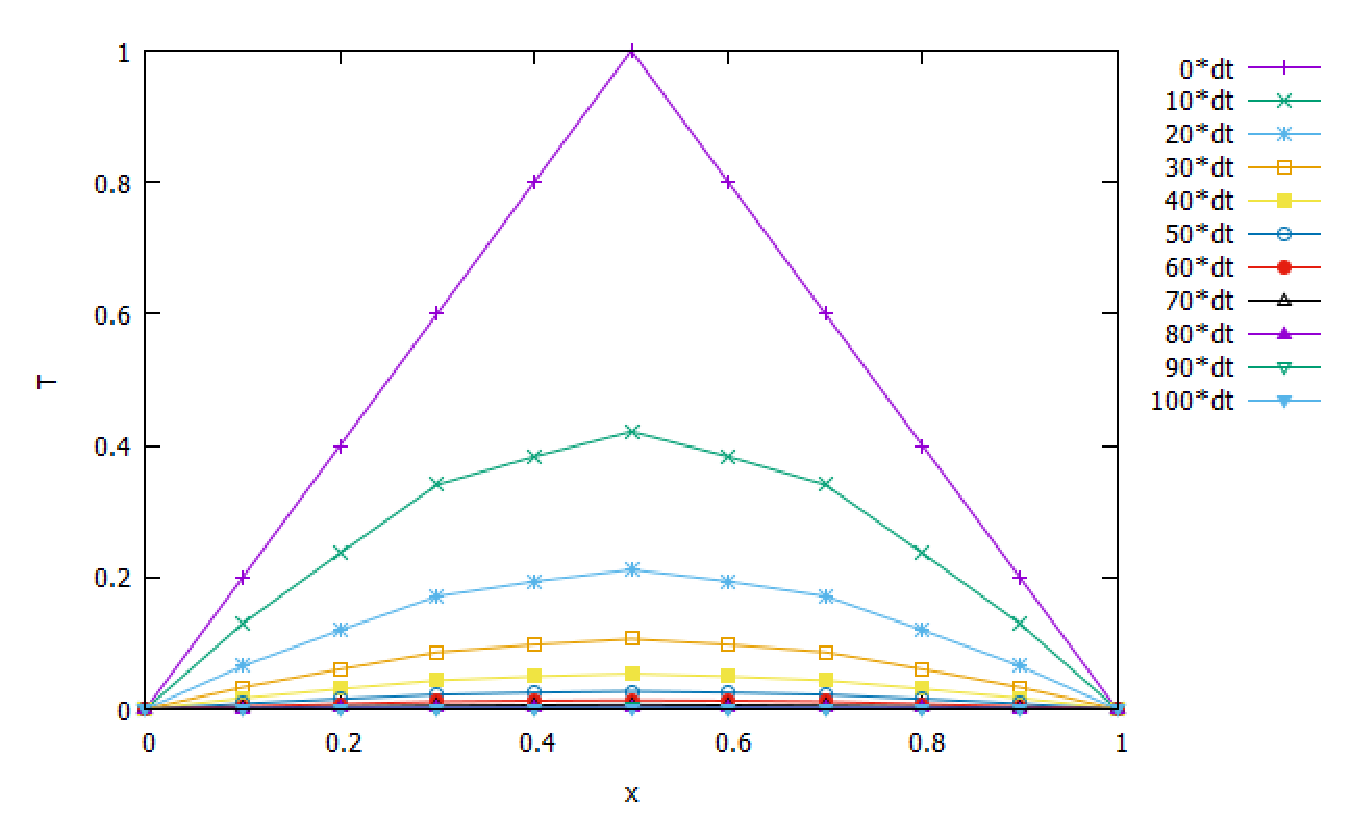
\includegraphics[width=14cm]{pic04.eps}
	\caption{Bloch磁壁の磁化構造}
	\label{fig04}
\end{figure}
\begin{figure}[H]
	\centering
	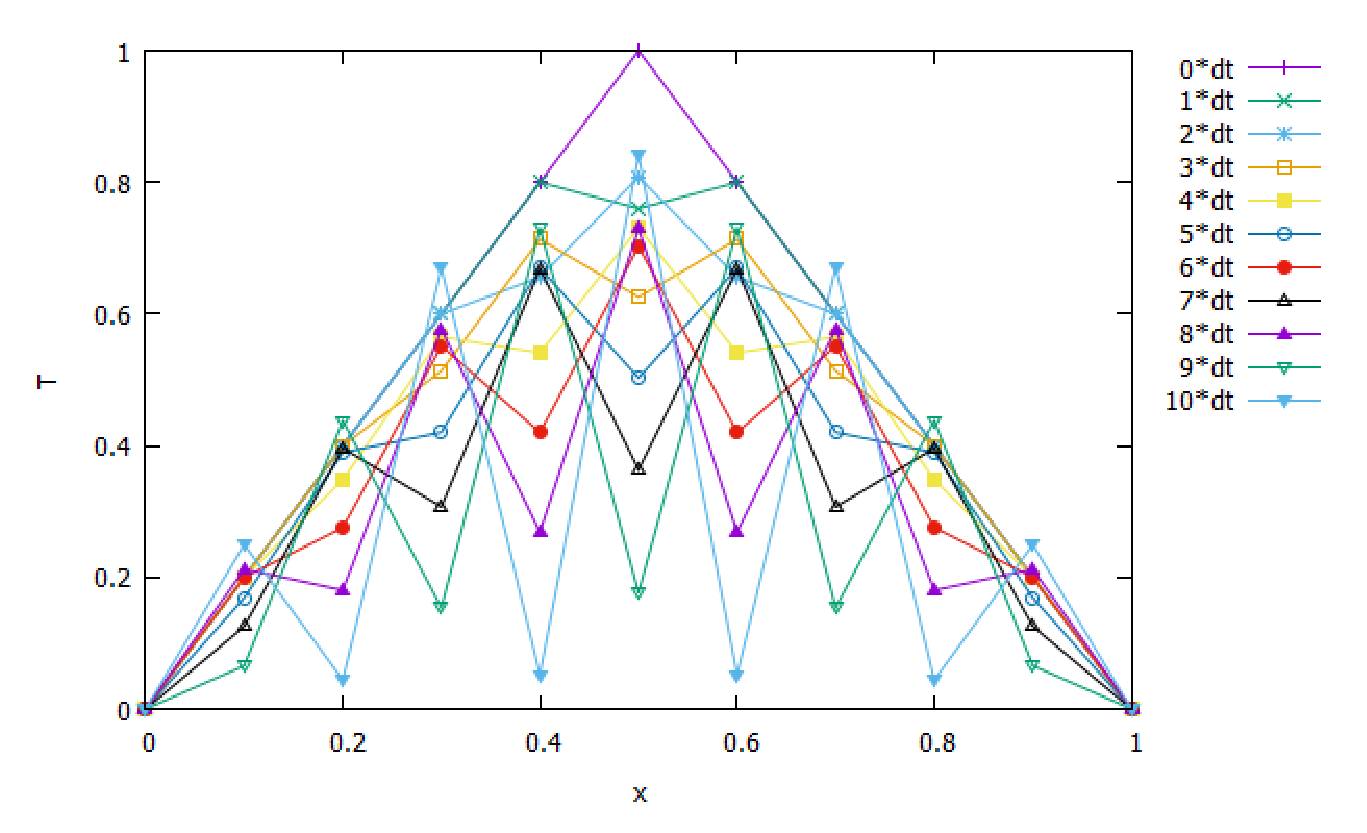
\includegraphics[width=14cm]{pic05.eps}
	\caption{$\mathrm{N\Acute{e}el}$磁壁の磁化構造}
	\label{fig05}
\end{figure}

これらの結果から、磁壁幅を計算すると、Bloch磁壁では$lw_{sim} = 21.77785\;\mathrm{nm}$となり、
$\mathrm{N\Acute{e}el}$磁壁では$lw_{sim} = 45.96424\;\mathrm{nm}$となった。
このことから、$\mathrm{N\Acute{e}el}$磁壁の磁壁幅はBloch磁壁の磁壁幅よりも小さく、
原理で述べたような結果が得られた。


\section{参考文献}

\begin{itemize}
  \item 配布されたテキスト
\end{itemize}

\end{document}